\appendix
\chapter{Spuštění webové aplikace}
\label{startapp}
Pro základní spuštění aplikace lokálně je potřeba mít nainstalované na zařízení následující software:
\begin{itemize}
    \item .NET 6.0 a vyšší\footnote{.NET 6.0 dostupné z \url{https://dotnet.microsoft.com/en-us/download/dotnet/6.0}}
    \item Node.js v17.9.0. a vyšší\footnote{Node.js dostupné z \url{https://nodejs.org/en/download/}}
    \item Docker Compose, který je součástí Docker Desktop, verze 4.7.0 a vyšší\footnote{Docker Desktop: \url{https://docs.docker.com/compose/install/}}
\end{itemize}

Zdrojové soubory jsou dostupné z paměťového média přiloženého k bakalářské práci. Pokud máte v plánu využít médium, zkopírujte soubory z něj soubory na pevný disk vašeho počítače, jinak nelze zajistit funkcionalitu. 

Další možnost získání aplikace je naklonování repozitáře bakalářské práce z \url{https://github.com/Tricer121/BP}. 

\section{Kompilace a spuštění}
Kompilace je jednoduchá díky využítí \emph{Dockeru}. 
Pro spuštění stačí navigovat do kořenového adresáře práce, kde se nachází soubor \emph{docker-compose.yml}. Následně proveďte dva příkazy:
\begin{itemize}
    \item docker compose build
    \item docker compose up
\end{itemize}

V konzolové řádce se vám zobrazí adresa, na které běží frontend aplikace\,--\,\url{http://localhost:8080}. Backend běží na portu 7040, což není ovšem pro spuštění relevantní informace.

\section{Spuštění po červenci 2022}
I lokální instance aplikace se spoléhá na existenci vzdáleného serveru s databází \emph{MySQL} a \emph{Overpass API}. Pokud máte zájem znovu zprovoznit aplikaci, můžete mě kontaktovat nebo postupovat dle informací v sekci \ref{serversetup}, která popisuje nastavení serveru. Poté je potřeba upravit soubor \emph{./backend/appsettings.json} s novou URL serveru databáze.
\chapter{Obsah paměťového média}
Adresářová struktura paměťového média je následovná:
{\small
%
\dirtree{%.
.1 /\DTcomment{kořenový adresář média}.
.2 docker-compose.yml\DTcomment{konfigurační soubor dockeru}.
.2 latexsrc\DTcomment{složka se zdrojovým kódem BP}.
.2 backend\DTcomment{adresář serverové části aplikace}.
.3 Classes\DTcomment{pomocné třídy}.
.3 Common\DTcomment{pomocné enumy}.
.3 Migrations\DTcomment{databázové migrace}.
.3 Models\DTcomment{definice entit pro EF}.
.3 Repositories\DTcomment{}.
.3 AppDbContext.cs\DTcomment{}.
.3 Dockerfile\DTcomment{kompilační soubor dockeru}.
.3 Program.cs\DTcomment{předvolený soubor ASP.NET aplikací}.
.3 appsettings.json\DTcomment{konfigurační uživatelský soubor}.
.2 frontend\DTcomment{adresář klientské části aplikace}.
.3 src.
.4 assets\DTcomment{použité obrázky}.
.4 components\DTcomment{jednotlivé komponenty}.
.4 models\DTcomment{použité třídy}.
.4 plugins\DTcomment{}.
.4 router\DTcomment{Vue směrování}.
.4 services\DTcomment{Služby}.
.4 store\DTcomment{}.
.4 styles\DTcomment{definované barvy, proměnné, písmo}.
.4 views\DTcomment{jednotlivé stránky}.
.4 App.vue\DTcomment{}.
.4 main.ts\DTcomment{konfigurační soubor}.
.3 Dockerfile\DTcomment{kompilační soubor dockeru}.
.3 index.html\DTcomment{základní stránka aplikace}.
.3 package.json\DTcomment{konfigurační soubor Vue}.
.2 osm zpracovani\DTcomment{skripty pro výpočet Voroného regionů}.
.3 extract\_nodes\_from\_osm.py\DTcomment{skript k extrakci dat z .osm souboru}.
.3 run\_voronoi.py\DTcomment{skript pro výpočet Voroného regionů}.
}
}
\chapter{Použití SQL Studia}
\label{sqlserverpictures}
\begin{figure}[h]
    \centering
    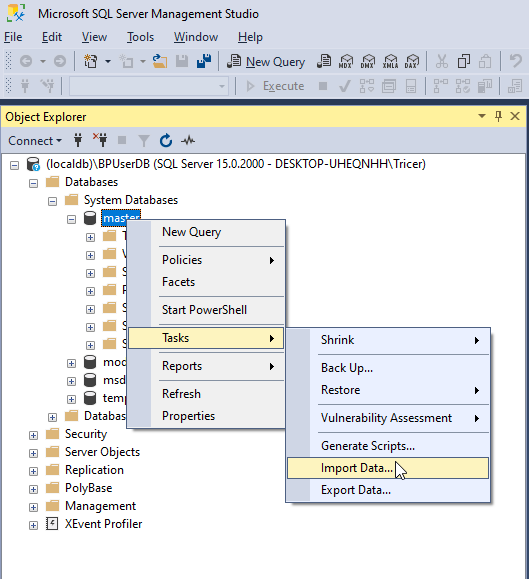
\includegraphics[width=0.9\textwidth]{obrazky/studio_1.png}
    \caption{Kontextové menu v SQL Server Management Studiu}
    \label{studio_1}
\end{figure}
\begin{figure}[h]
    \centering
    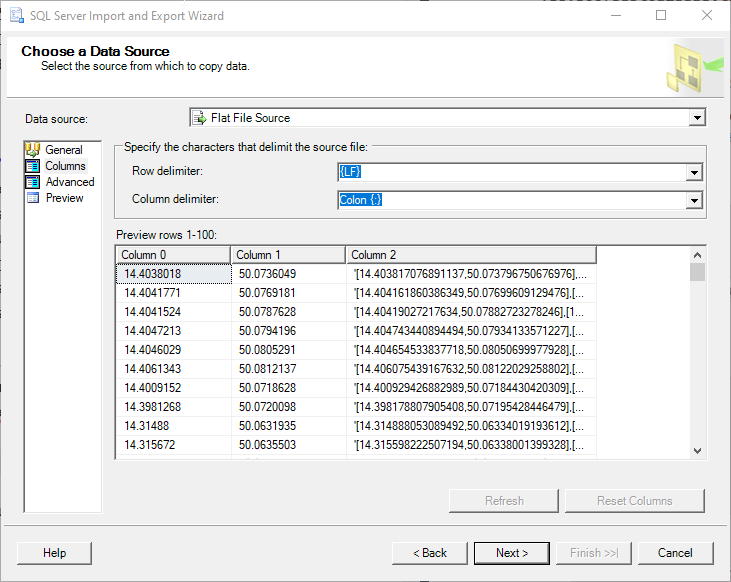
\includegraphics[width=1\textwidth]{obrazky/studio_2.png}
    \caption{Rozdělení dat do sloupců v SQL Server Management Studiu}
    \label{studio_2}
\end{figure}
\chapter{Testování aplikace}
\label{test:app}
\begin{figure}[h]
    \centering
    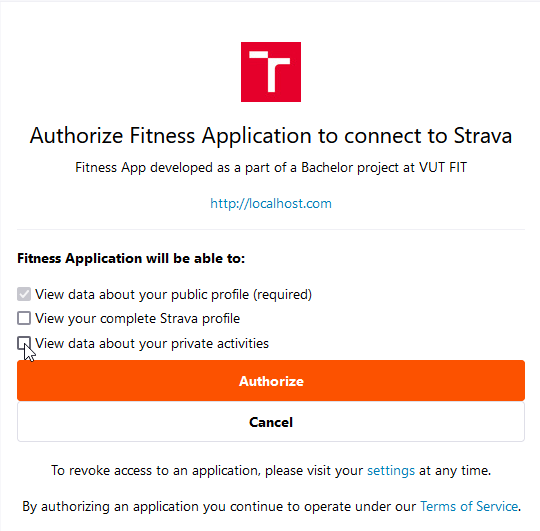
\includegraphics[width=0.7\textwidth]{obrazky/test_loginbadperm.png}
    \caption{Špatně nastavené povolení uživatele v aplikaci Strava}
    \label{test:login_cancel}
\end{figure}
\begin{figure}[h]
    \centering
    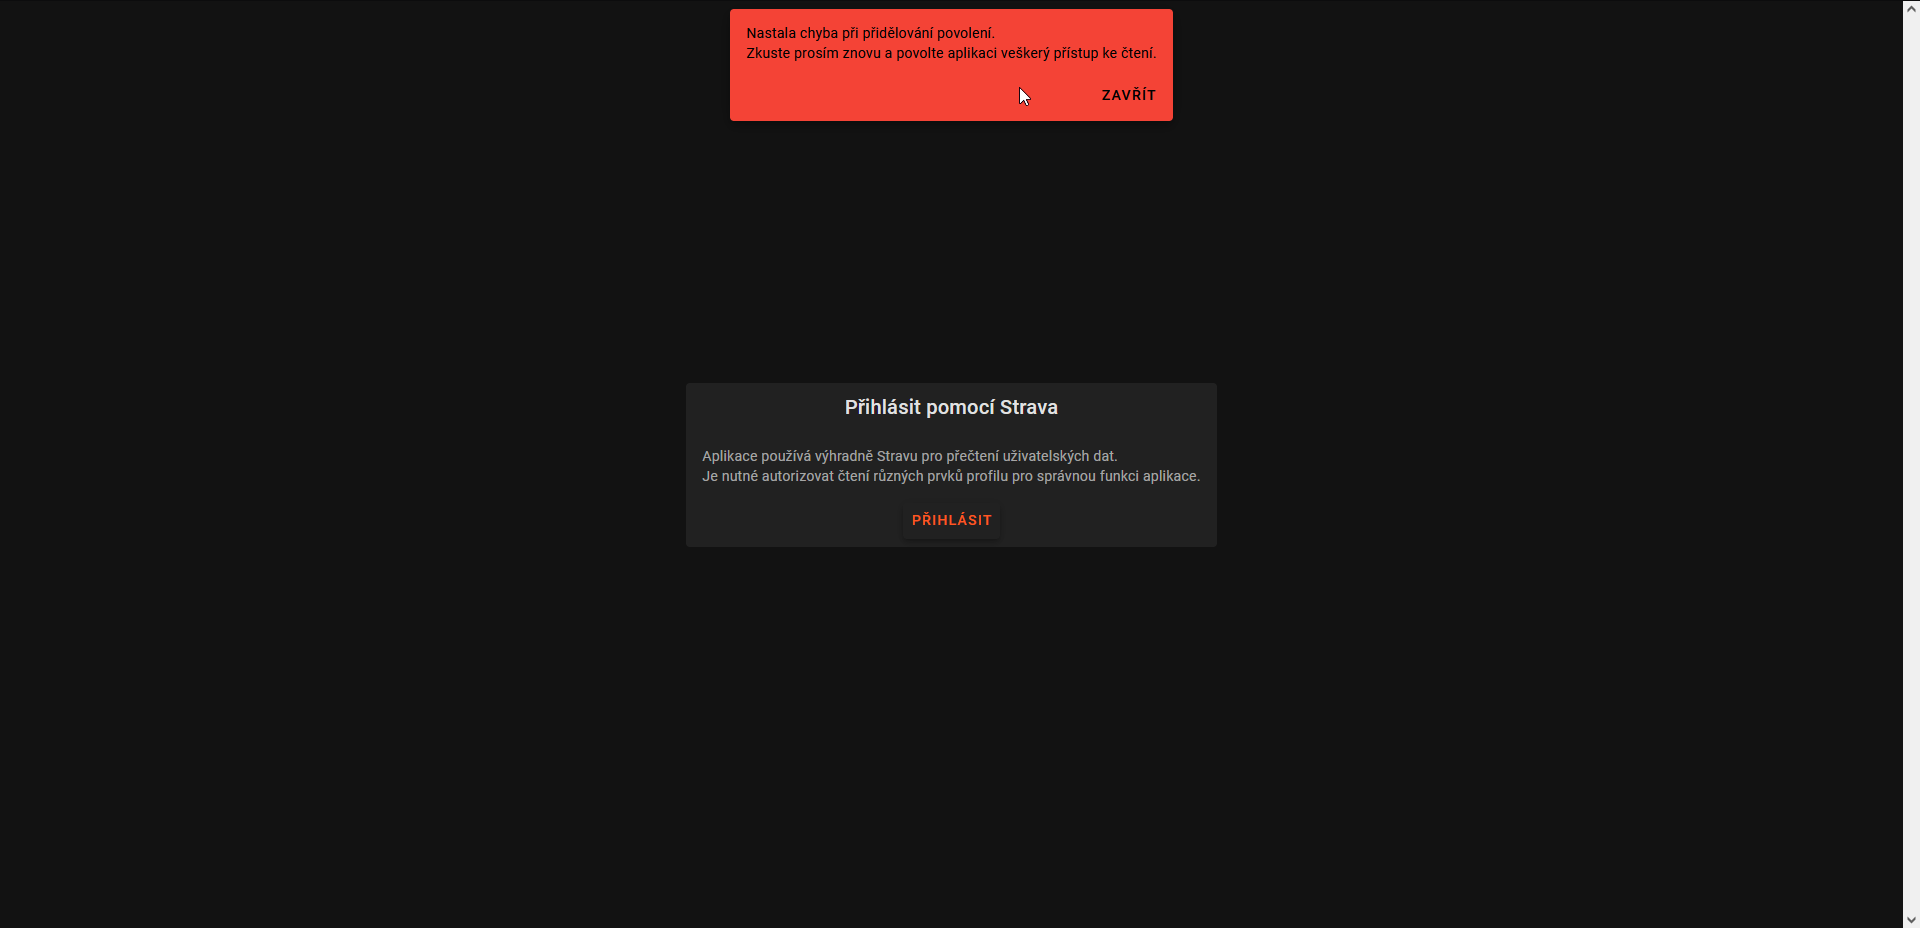
\includegraphics[angle=90,width=0.7\textwidth]{obrazky/test_faillogin.png}
    \caption{Selhání přihlášení uživatele}
    \label{test:login_fail}
\end{figure}
\begin{figure}[h]
    \centering
    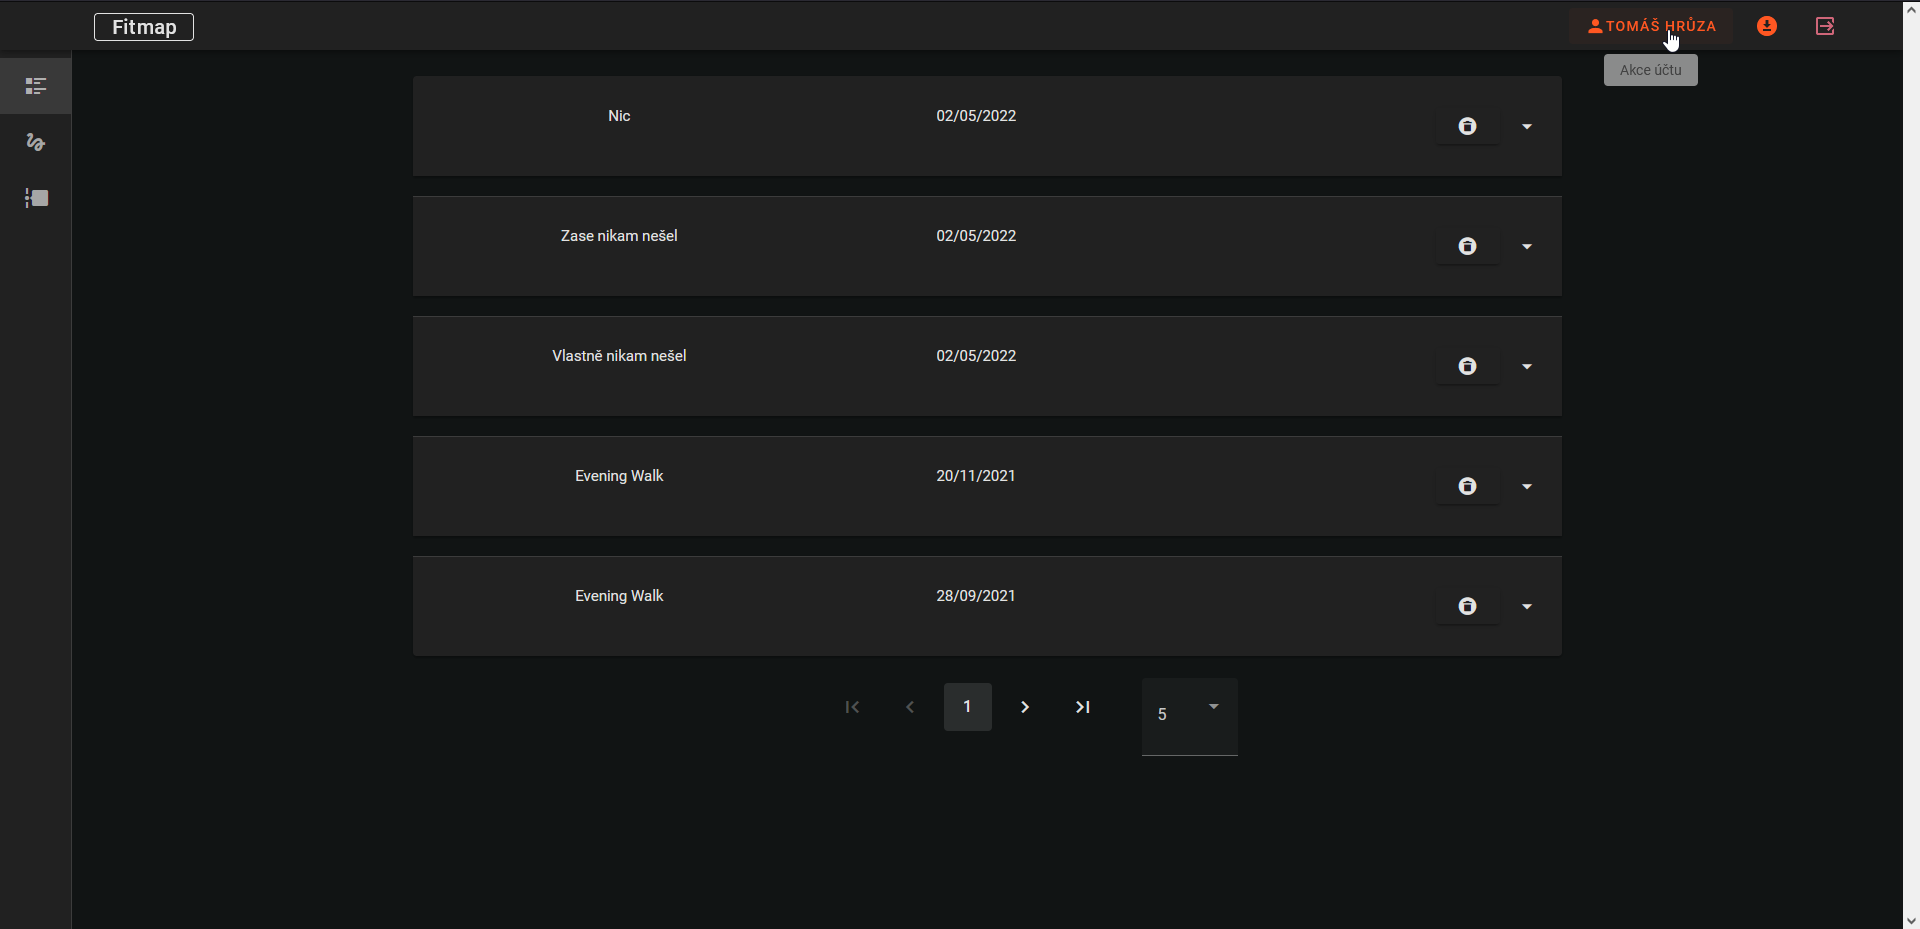
\includegraphics[angle=90,width=0.7\textwidth]{obrazky/test_activitylist.png}
    \caption{Seznam aktivit}
    \label{test:activity_list}
\end{figure}
\begin{figure}[h]
    \centering
    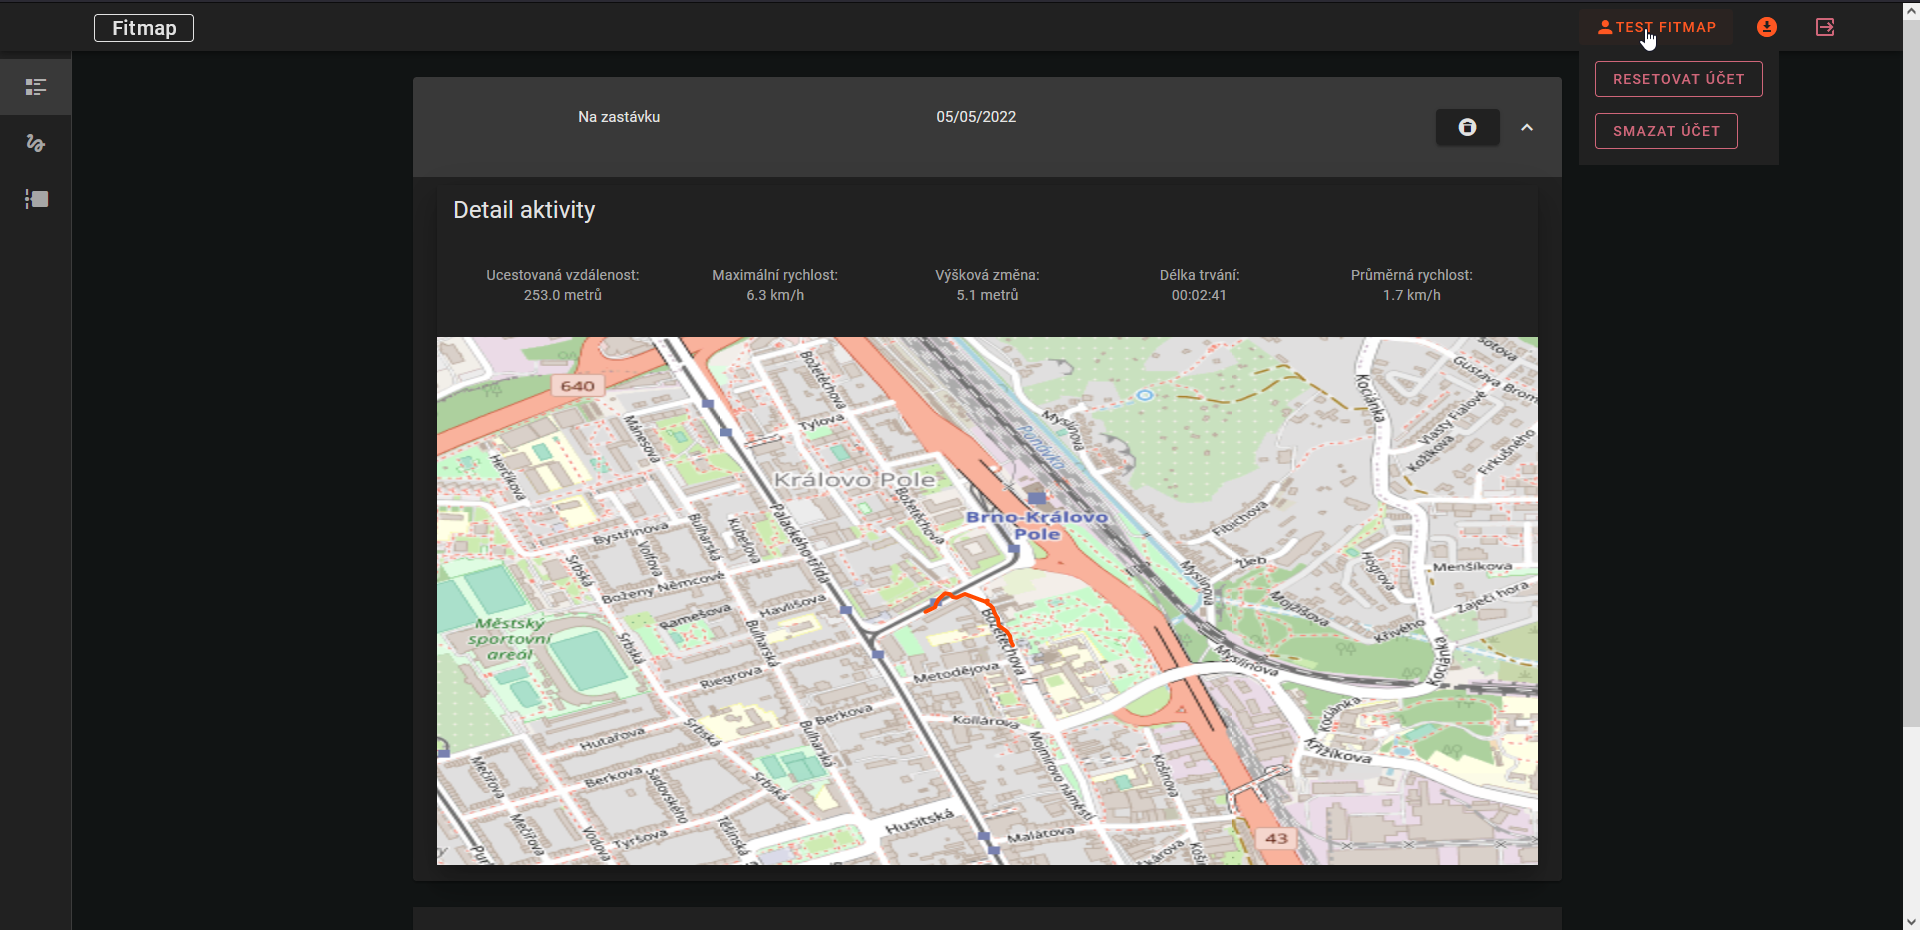
\includegraphics[angle=90,width=0.7\textwidth]{obrazky/test_activitydetail.png}
    \caption{Detail aktivity}
    \label{test:activity_detail}
\end{figure}
\begin{figure}[h]
    \centering
    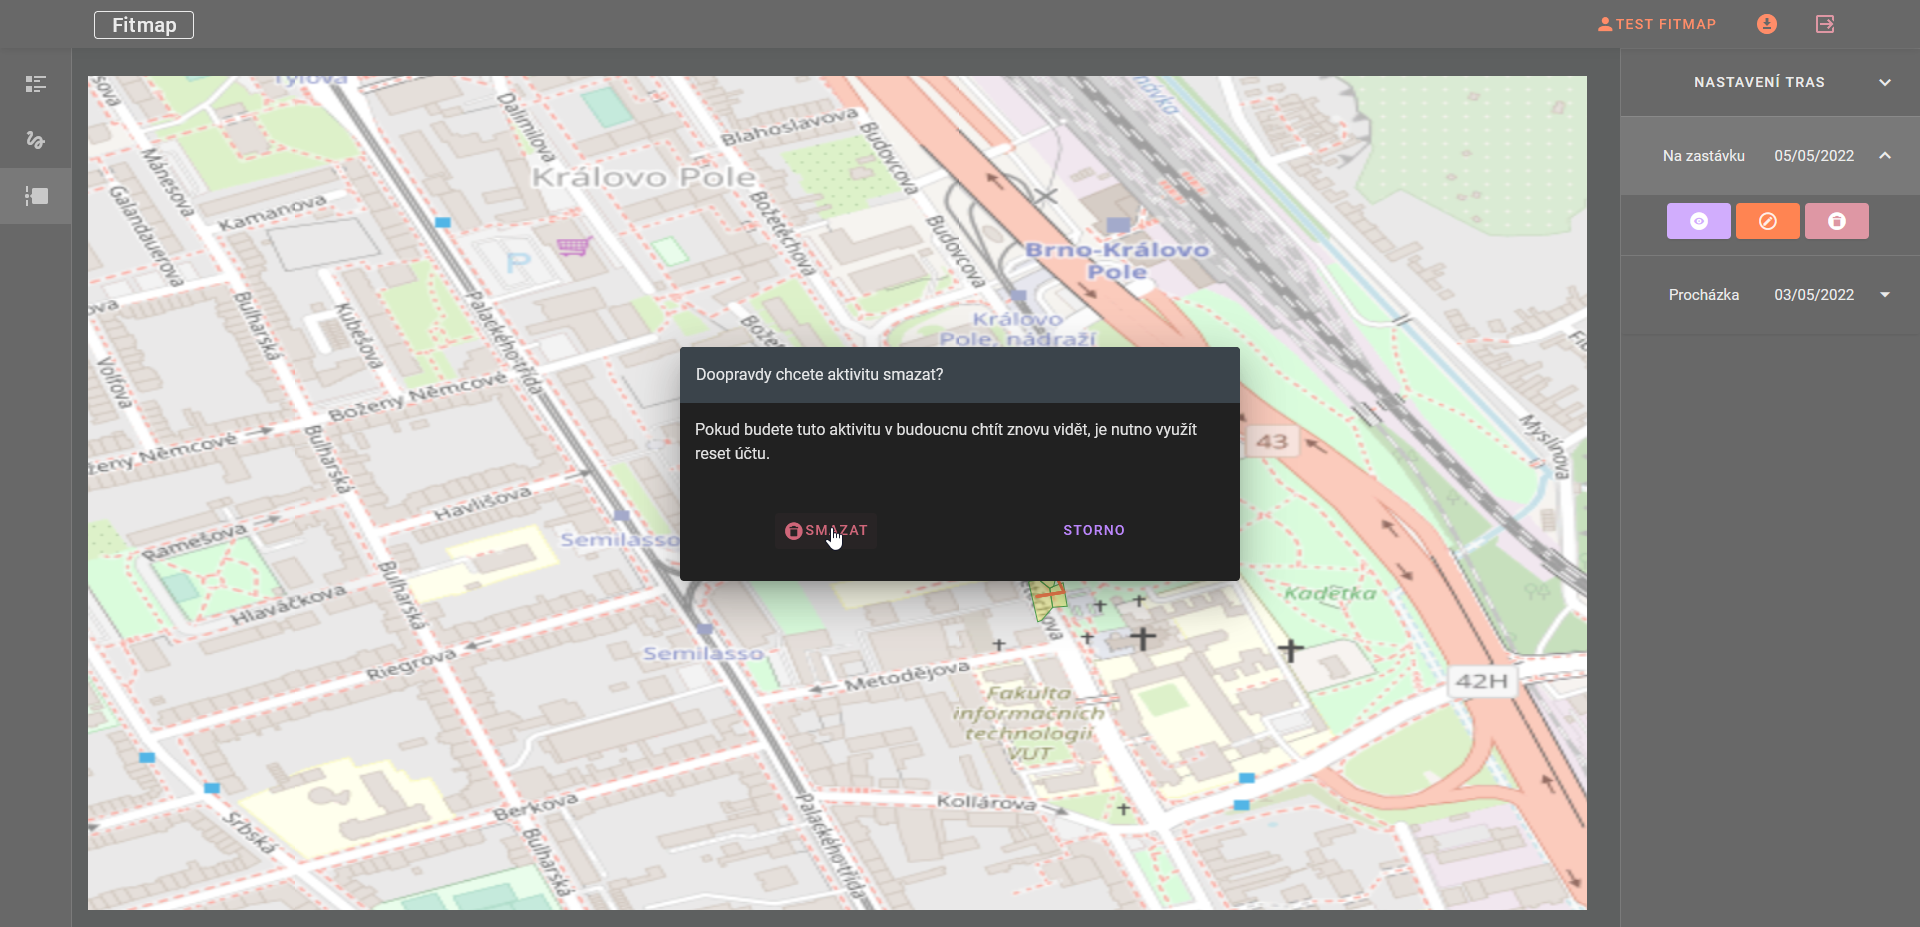
\includegraphics[angle=90,width=0.7\textwidth]{obrazky/test_dialog.png}
    \caption{Varovný dialog}
    \label{test:dialog}
\end{figure}
\begin{figure}[h]
    \centering
    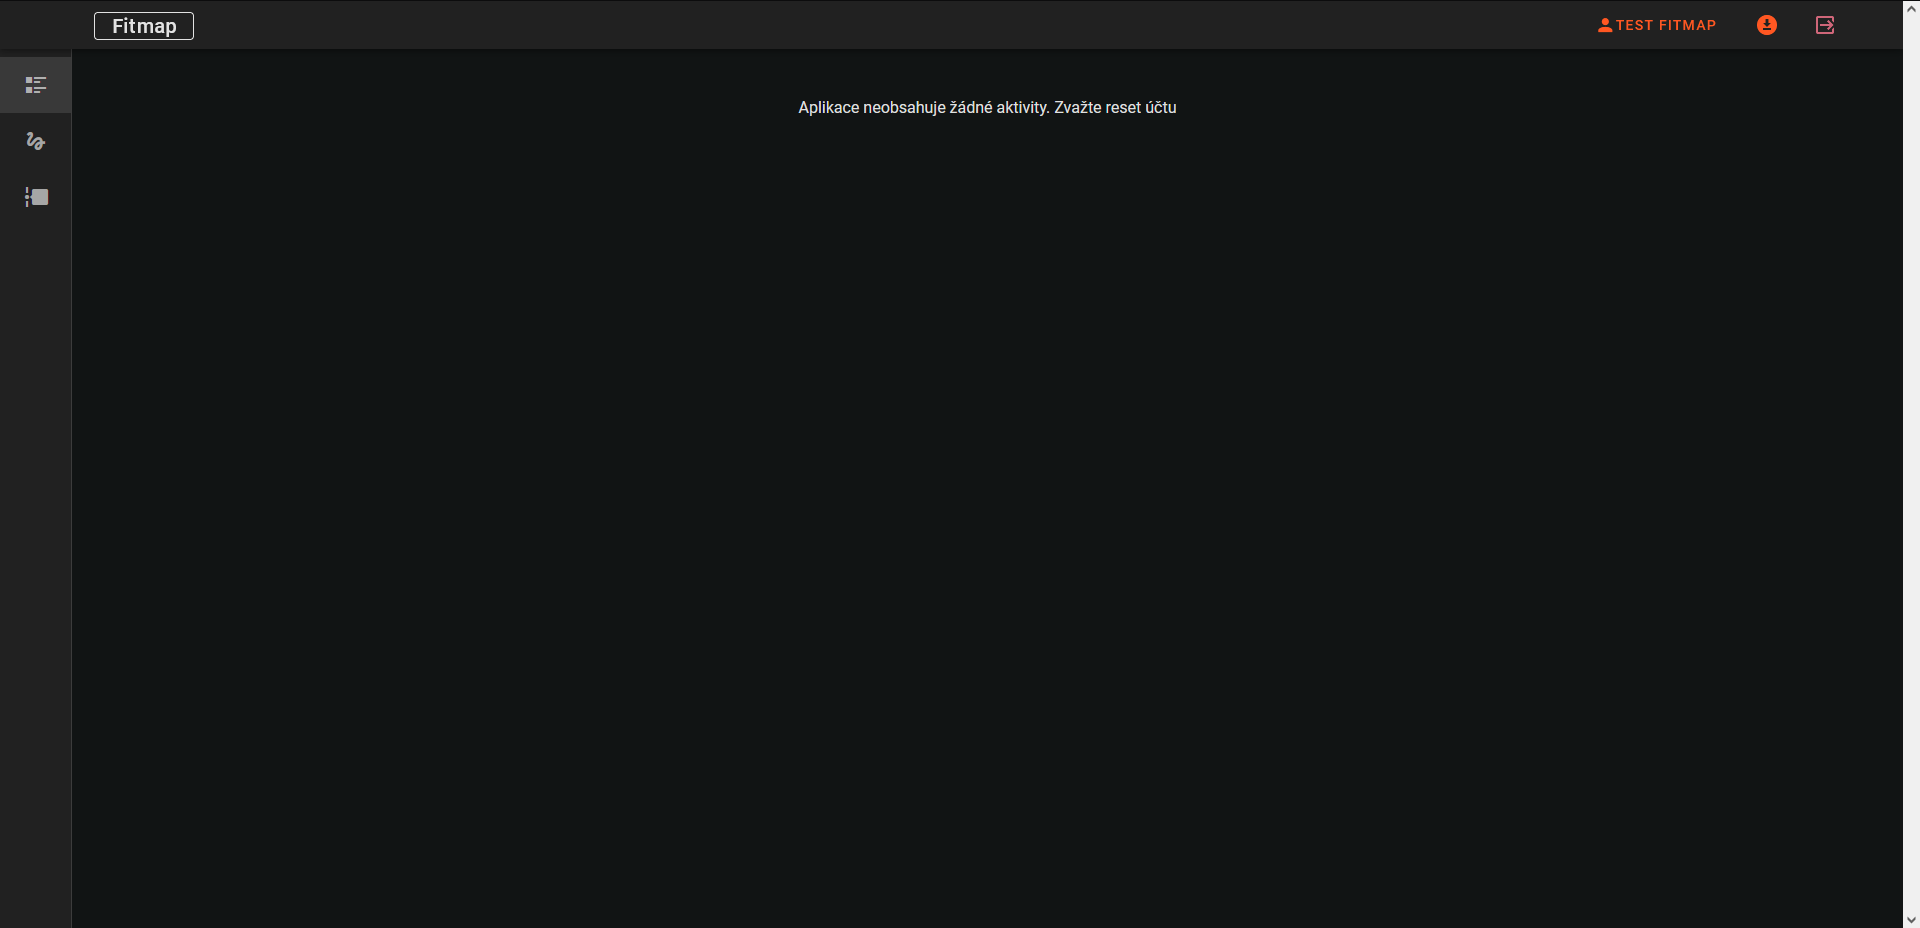
\includegraphics[angle=90,width=0.7\textwidth]{obrazky/test_appempty.png}
    \caption{Zobrazení bez aktivit na účtě}
    \label{test:app_empty}
\end{figure}
\begin{figure}[h]
    \centering
    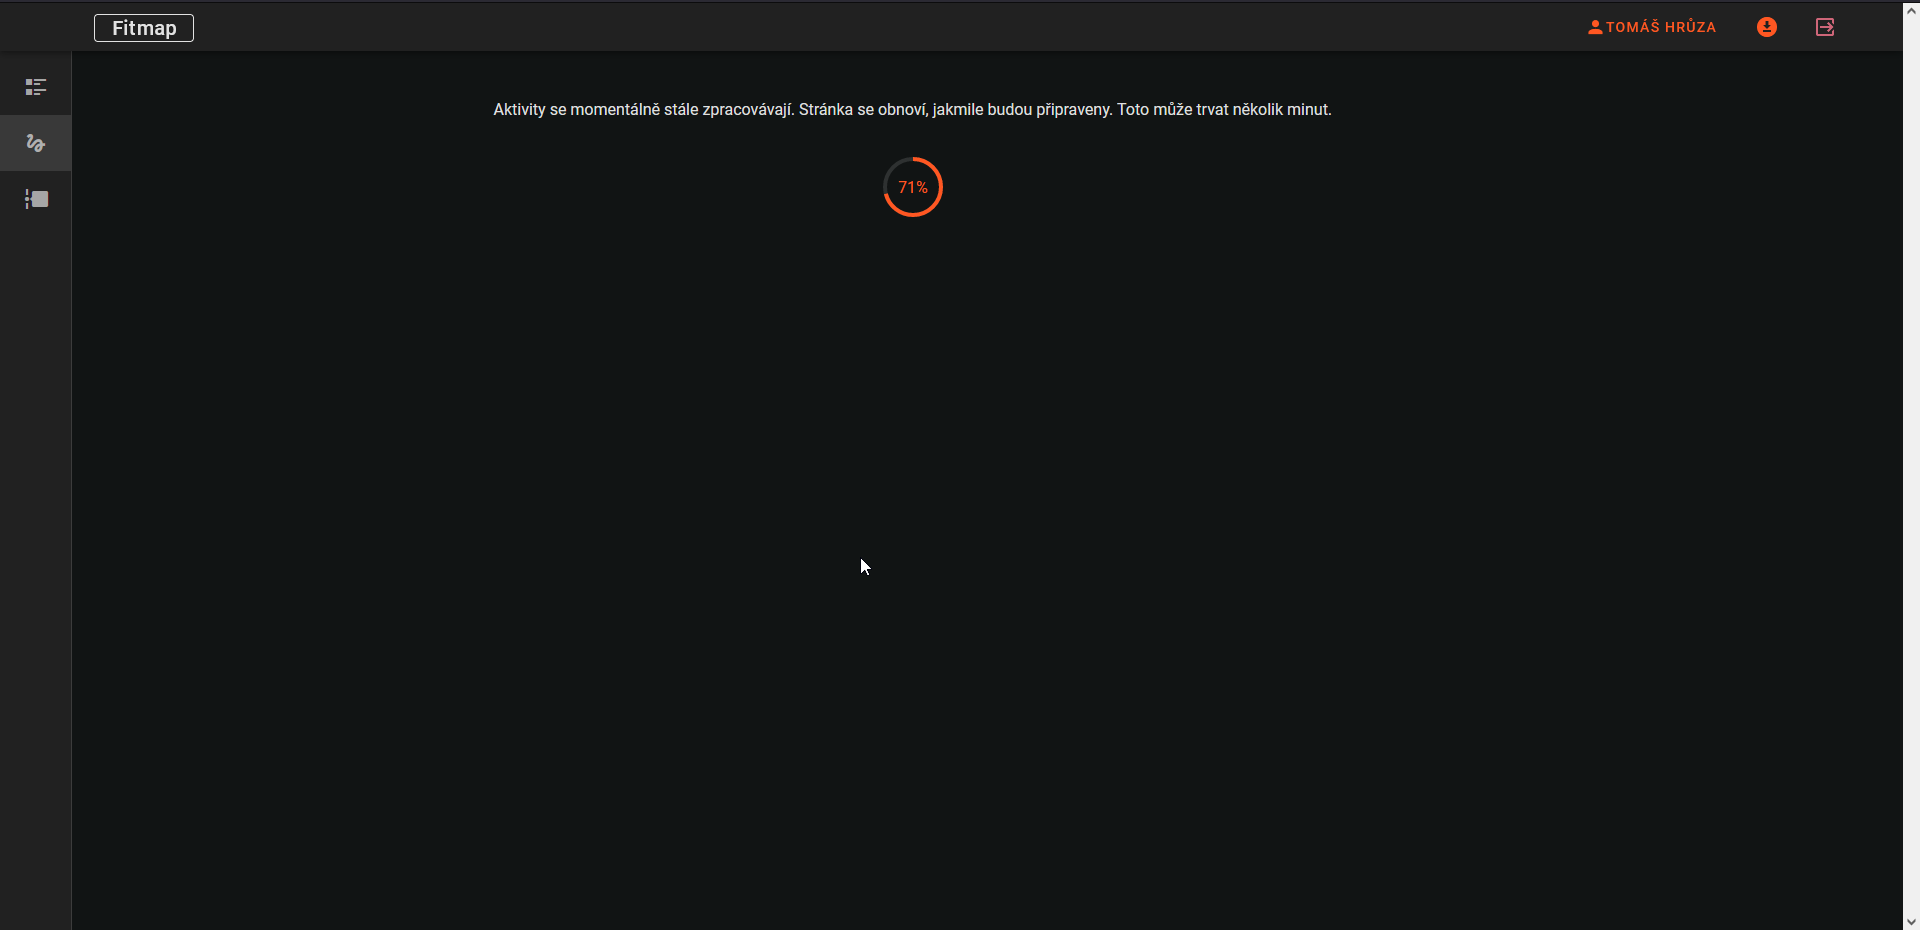
\includegraphics[angle=90,width=0.7\textwidth]{obrazky/test_loading.png}
    \caption{Načítací komponenta při zpracování aktivit}
    \label{test:loading}
\end{figure}
\begin{figure}[h]
    \centering
    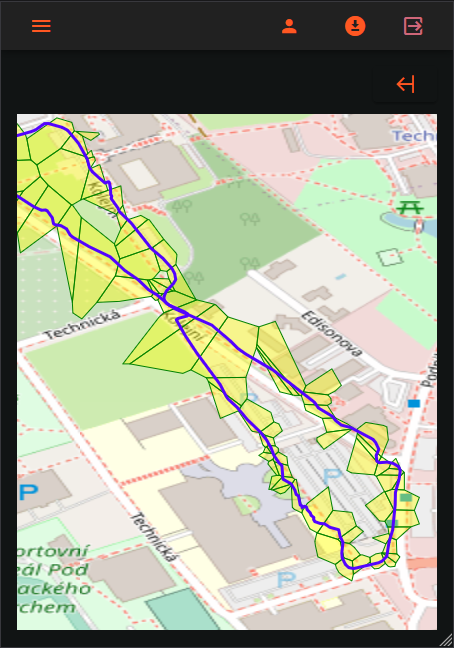
\includegraphics[width=0.7\textwidth]{obrazky/test_responsive.png}
    \caption{Responzivní zobrazení zabraného území}
    \label{test:responsive}
\end{figure}
\begin{figure}[h]
    \centering
    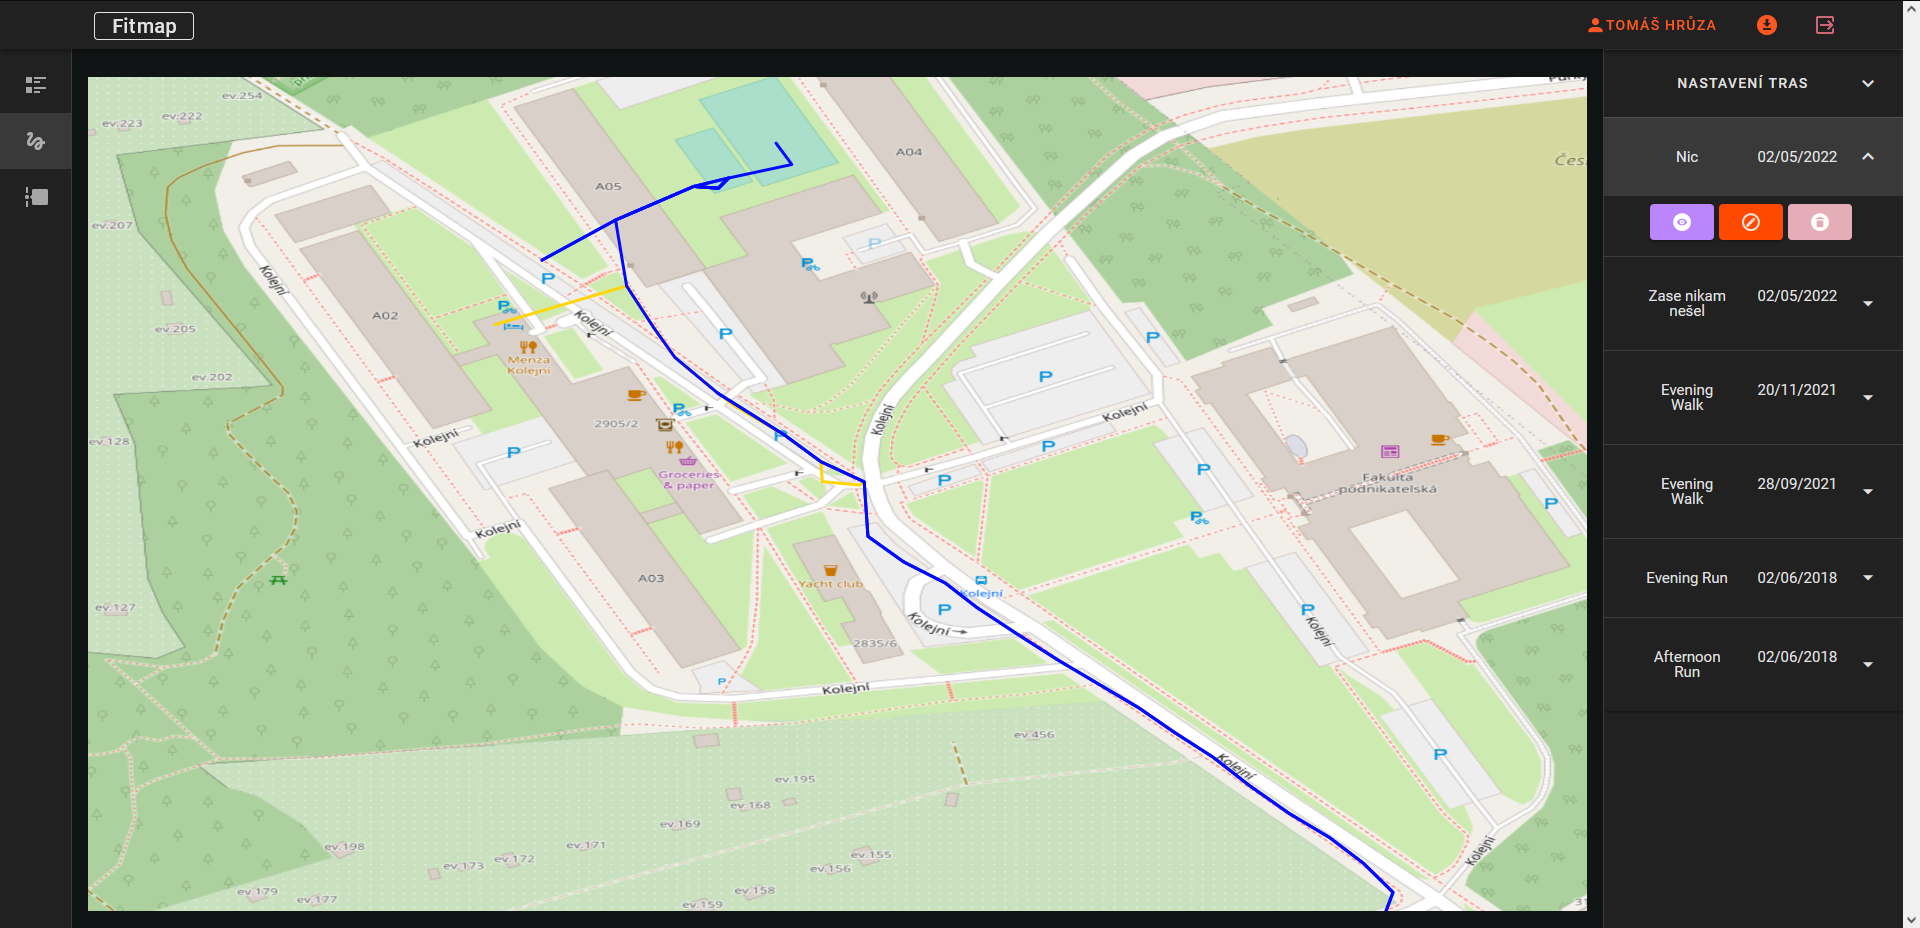
\includegraphics[angle=90,width=0.7\textwidth]{obrazky/test_filterAB.png}
    \caption{Filtrace tras}
    \label{test:filterAB}
\end{figure}

